% Project Topic Proposal — Shift-Left Accessibility (alternate wording, one figure)
\documentclass[12pt]{article}
\usepackage[left=1in,right=1in,top=1in,bottom=1in]{geometry}
\usepackage{setspace}
\usepackage{graphicx}
\singlespace

\title{\textbf{Shift-Left Accessibility for UX/UI: A Figma Preflight vs.Code-Time Checks (Pilot)}}
\author{Noelynn Faith Batalingaya}
\date{September 2025}

\begin{document}
\maketitle

\section*{Problem Statement \& Motivation}
My project starts from a simple, practical question: \emph{How much accessibility can we catch while the interface is still a Figma mockup, and does doing that early save time once we write code?} In real teams, accessibility often shows up late and creates rework. I want to test whether a short, repeatable "preflight" checklist during design reviews prevents common issues from ever reaching implementation.

\section*{Background \& Prior Work}
Accessibility is ultimately about real people being able to use what we ship—from screen reader and keyboard-only users to people with low vision, older adults, and anyone using a cracked phone outdoors. HCI research argues that inclusive design should start at the beginning, not as a last-minute checklist \cite{bennett2018inclusive}. Recent studies show that many problems are visible \emph{in the mockups} themselves—low color contrast, small hit targets, unclear component states, and weak hierarchy—and can be assessed systematically in Figma before any code exists \cite{huang2024a11yfigma, chen2024figmaapps}. Work with UX practitioners also highlights real barriers (time, ownership, uneven training) and recommends lightweight checklists and design-system constraints as realistic, adoptable improvements \cite{shi2023uxaccesspractice}. My pilot turns these insights into a small but measurable study.

\section*{Project Scope \& Goals}
\textbf{Goal 1.} Create a one-page \emph{Figma Accessibility Preflight} centered on five checks: (a) contrast \& legibility, (b) hierarchy \& structure, (c) target size \& spacing, (d) state visibility (focus/hover/active/disabled/error), and (e) basic semantics/affordances (labels, recognizable controls).\\
\textbf{Goal 2.} Implement two matching screens (Home + Register) as a tiny website and run code-time checks (keyboard, screen reader, automated tools).\\
\textbf{Goal 3.} Compare \emph{which issues are caught when} and the \emph{minutes to fix} at design vs.\ code time.

\textbf{Research Questions.} 
\textbf{RQ1:} Which issue types are reliably caught at design time versus only at code time (e.g., focus order, announcements)? 
\textbf{RQ2:} Does the preflight reduce “minutes to fix” compared to fixing after implementation?

\section*{Planned Software (what I will build)}
To keep effort manageable and the focus on accessibility (not tools), I will build a minimal two-page site using HTML/CSS plus a few lines of JavaScript:
\begin{itemize}
  \item \textbf{Home:} semantic landmarks (\texttt{header/nav/main/footer}), a visible \emph{Skip to main content} link, proper headings, high-contrast tokens, and a clear \texttt{:focus-visible} outline.
  \item \textbf{Register:} explicit \texttt{<label for>} on each field, hint text via \texttt{aria-describedby}, inline error messages with \texttt{role="alert"}, and focus moves to the first error on submit. All key interactions should work by keyboard (Tab/Shift-Tab/Enter/Space/Esc).
\end{itemize}

\section*{Method \& Measures}
\textbf{Phase A — Design-time Preflight.} I will run the five checks on two Figma mockups (Home, Register). For every issue, I will log: \texttt{screen\_id, phase=design, category, severity, found\_by=preflight, fix\_minutes, notes}. I'll then update the mockups and record the design fix minutes.

\textbf{Phase B - Code-time Checks.} I will build the two pages and perform three passes:
\begin{enumerate}
  \item \emph{Keyboard pass:} reach everything with Tab/Shift-Tab, visible focus, no traps, expected Enter/Space/Esc behavior.
  \item \emph{Screen reader pass (macOS VoiceOver):} names/roles/labels, headings/landmarks, and whether errors are announced.
  \item \emph{Automated audits:} Lighthouse and axe DevTools for quick, repeatable checks.
\end{enumerate}
Each issue will be logged with \texttt{phase=code} and \emph{code fix minutes}. 

\textbf{Analysis.} I will compare counts by phase and category and graph the average \emph{minutes to fix} at design vs.\ code. Based on prior work, I expect the preflight to catch many visual/structural issues quickly while code-time checks remain essential for focus order and screen reader announcements \cite{huang2024a11yfigma, chen2024figmaapps, shi2023uxaccesspractice}. I will discuss limits (small pilot, student context) and outline how to expand next semester (more screens; possibly recruit assistive technology users; compare teams with vs.\ without the preflight).

\section*{Illustration (logic only)}
This proposal includes one figure: a logic diagram summarizing the flow from the Figma preflight to code-time checks and the final comparison of issues and fix minutes (Figure~\ref{fig:logic}).

\begin{figure}[h]
  \centering
  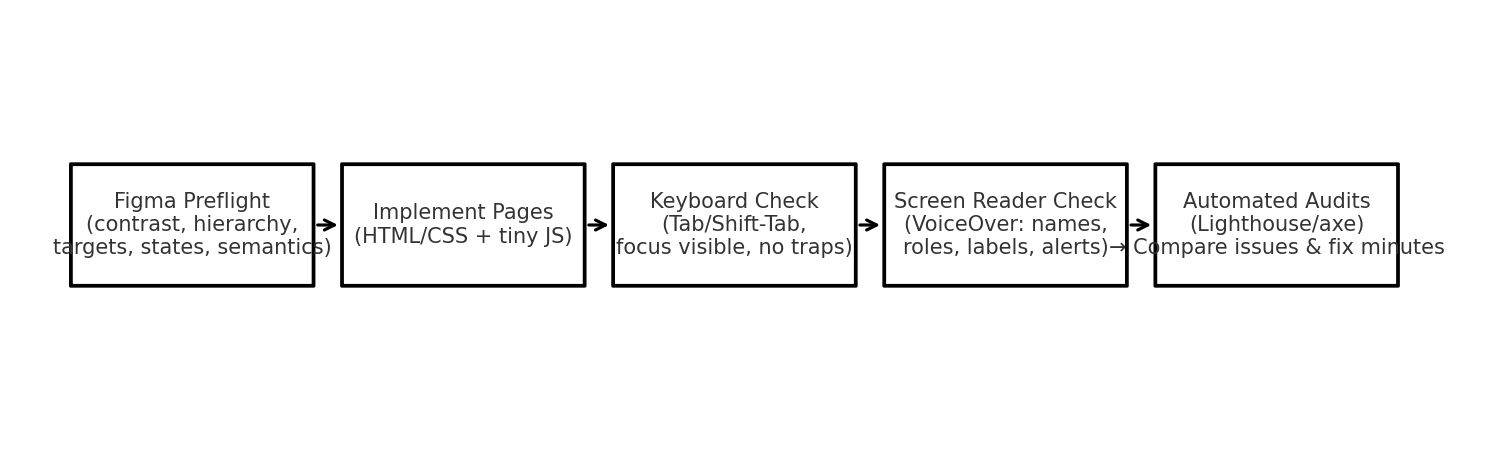
\includegraphics[width=0.95\linewidth]{figs/logic-diagram.png}
  \caption{Workflow: Preflight on mockups $\rightarrow$ Implement pages $\rightarrow$ Keyboard/Screen Reader/axe checks $\rightarrow$ Compare issues \& fix minutes.}
  \label{fig:logic}
\end{figure}

\section*{Expected Contributions}
Deliverables will include: (1) a short, printable preflight that can be used in design critique; (2) a tiny set of accessible component patterns (focus ring, skip link, labeled inputs, reduced motion); and (3) a small dataset that shows where early checks save time and where code-time checks are still required. These are practical outcomes for student teams and a solid foundation to scale into a larger Senior IS.

\bibliographystyle{acm}
\bibliography{bibliography.bib}

\newpage
\section*{Appendix: Feature List (implementation order)}
\begin{enumerate}
  \item Add semantic landmarks and a \emph{Skip to main content} link.
  \item Set heading hierarchy (H1/H2/H3) and spacing scale.
  \item Add a clear \texttt{:focus-visible} outline (high contrast, offset).
  \item Define color tokens and verify contrast (text \& UI) against WCAG AA.
  \item Build \textbf{Home} navigation: keyboard-reachable links; hover/active states; visible focus.
  \item Build \textbf{Register} form with \texttt{<label for>} and hint text via \texttt{aria-describedby}.
  \item Inline error message with \texttt{role="alert"} and focus-to-first-error on submit.
  \item Enforce \textbf{target size} minimums ($\sim 44\times 44$ px) and adequate spacing between controls.
  \item Respect \texttt{@media (prefers-reduced-motion)} for users who limit animation.
  \item Run Lighthouse/axe; log issues + \emph{fix\_minutes}; capture before/after screenshots.
  \item[\textit{Stretch}] Add a basic \textbf{table pattern} (caption, header cells with scope) + one-sentence text summary.
  \item[\textit{Stretch}] Add a short \textbf{alt-text guide} and test a tiny image gallery (good vs.\ poor examples).
  \item[\textit{Stretch}] Optional automation: run Pa11y or jest-axe locally for quick regression checks.
\end{enumerate}

\end{document}
